\chapter{连续血糖预测}\label{chap:predict}

毛细血管全血糖检测(Capillary Blood Glucose, CBG)是一种常用的患者自测使用的血糖检测方法,该技术通过袖珍血糖仪可以迅速、便捷地测量患者的血糖水平. 这种技术赋予糖尿病患者能力,使他们可以在家中自行监测血糖,及时了解自身的血糖情况,从而及时调整治疗方案. 

CBG检测的原理是利用葡萄糖氧化酶的比色反应. 在这一过程中,葡萄糖氧化酶作为催化剂,将葡萄糖氧化为葡萄糖酸和过氧化氢. 随后,由于过氧化氢同时具有氧化性和还原性,会分解为氧气和水,而生成的氧气可以使测试剂的颜色发生变化. 这种变化可以通过光度计或吸收光度计来测定,也可以使用电化学方法测定产生的电流来获取血糖值. 

CBG检测技术的优势在于操作简单、结果快速可得,适合患者进行自我血糖监测. 然而,它也有一些局限性,例如会受到血细胞比积的影响,以及由于是患者独立操作可能存在操作不当或仪器质量问题导致的误差. 

在医疗实践中,CBG检测是糖尿病患者日常血糖管理的关键工具之一. CGM技术作为CBG检测的补充,能够提供更全面的血糖信息,帮助患者更好地了解血糖变化趋势,发现潜在的高血糖和低血糖情况. 

在实践中,为了得到更为准确的血糖数据,通常会两种技术同时使用,帮助患者更准确地认识到自己的血糖情况,从而更好地控制糖尿病. 

\section{连续血糖监测技术}
CGM技术与传统的间断性血糖检测相比,CGM技术能够提供更加精确和详细的血糖数据,并且可以给出随时间变化的血糖波动曲线,这可以帮助患者更好地了解自己的血糖波动情况,并及时调整胰岛素剂量或饮食习惯. 

CGM技术通常由一个植入皮肤下的葡萄糖传感器和一个便携式的数据接收器组成. 传感器定期测量组织液中的葡萄糖浓度,并将数据传输到接收器上. 接收器可以显示实时血糖数据,或者将数据传输到手机或计算机上进行进一步分析和记录. 

通过CGM技术,糖尿病患者可以实时监测到血糖的波动情况,及时发现低血糖或高血糖的风险,并采取相应的措施进行调整. 此外,CGM技术还可以提供血糖趋势预测和报警功能,帮助患者更好地管理血糖\cite{vigersky2017role}. 

近年来,随着CGM技术的不断发展和改进,越来越多的糖尿病患者选择使用CGM技术来管理他们的血糖. CGM技术的广泛应用为糖尿病管理提供了新的思路和方法,有望进一步改善患者的生活质量和健康状况. 
\section{数据处理}
从收集到的病人血糖数据\cite{zhao2023chinese}中可以发现,病人服用与胰岛素有关的药物以及进食一般是同时进行的,因此可以将进食视为以此扰动,以每次进食为界线,在这之后当病人的血糖达到局部极值开始,我们视为没有其他外界葡萄糖,胰岛素等摄入,知道下一次进食,这一整组数据整合为$(G_i,t_i)_{i=1}^n$,其中$G_i$为血糖浓度, $t_i$为时间. 通过这组数据,我们用梯度下降法求解出对应病人的最优参数,以此作为我们的模型参数. 我们就可以通过此模型对该病人某次进食后的初值对他后续血糖值做预测,并且可以根据对应的参数值大小来推测病人的病情以及制定个性化治疗方案. 

同时,我们也要衡量具体扰动的大小,由于我们只知道病人吃了什么,并没有确切的葡萄糖和胰岛素变化数值,因此我们使用薄荷健康的数据,将病人每次的进食数据转换为卡路里,葡萄糖等数据,再配上服用药物中含有的胰岛素等数据,以此作为扰动的大小. 
\section{动力系统模型的选择以及训练}
我们采用两种模型来进行连续血糖预测,分别是模型\ref{model1}:
\begin{equation}\label{model1}
    \begin{aligned}
        \dot{G} & = a_0-a_1G-a_2GI+\frac{a_3}{a_4+I^p},  \\
        \dot{I} & = \frac{b_1 G^2}{G^2 + b_2^2} - b_3 I,
    \end{aligned}
\end{equation}
和模型\ref{model2}:
\begin{equation}\label{model2}
    \begin{aligned}
        \dot{G} & = a_0-a_1G-a_2GI,  \\
        \dot{I} & = \frac{b_1 G^2}{G^2 + b_2^2} - b_3 I,
    \end{aligned}
\end{equation}

其中模型\ref{11}是一个更加复杂的模型,其多考虑了人体自身的糖原储备,算上了肝糖原水解对血糖的影响,而模型\ref{model2}则是一个更加简单的模型,由于人体肝糖原水解产生的葡萄糖并不占很多部分,但考虑这部分却需要多引入三个参数,由于对同一个人的数据有限,参数越少训练效果越好,因此选择模型\ref{model2}也是合理的. 我们将通过训练这两个模型,来比较它们的预测效果. 

对于模型\ref{model1},我们先分析其稳定性. 
\begin{prop}
    模型\ref{model1}有唯一不动点,且该不动点为吸引子. 
\end{prop}

\begin{pf}
    为寻找该模型不动点,我们考查:
    \begin{equation}
        a_0-a_1G^*-a_2G^*I^*+\frac{a_3}{a_4+(I^*)^p}= \frac{b_1 (G^*)^2}{(G^*)^2 + b_2^2} - b_3 I^*=0,
    \end{equation}
    可以注意到:
    \begin{equation}
        I^*=\frac{b_1 (G^*)^2}{b_3((G^*)^2 + b_2^2)},
    \end{equation}
    显然$I^*$关于$G^*$是单调递增的,因此若$G^*$是唯一的则$I^*$是唯一的. 考虑函数$h(G)$
    \begin{equation}
        h(G)=a_0-a_1G-a_2G\frac{b_1G^2}{b_3(G^2+b_2^2)}+\frac{a_3(b_3^p(G^2+b_2^2)^p)}{a_4(b_3^p(G^2+b_2^2)^p+b_1^pG^{2p})},
    \end{equation}
    可以得出$h(G)$单调递减,且$h(0)>0,\lim_{G\to\infty}h(G)<0$,易得$\exists !G^*$使得$h(G^*)=0$因此,模型\ref{model1}有唯一不动点. 

    在点$(G^*,I^*)$处线性化模型\ref{model1},我们有:
    \begin{equation}\label{14}
        \begin{pmatrix}
            \dot{G} \\
            \dot{I}
        \end{pmatrix}=\begin{pmatrix}
            -a_1-a_2I^*                              & -a_2G^*-\frac{pa_3(I^*)^{p-1}}{(a_4+(I^*)^p)^2} \\
            \frac{2b_1b_2^2G^*}{((G^*)^2 + b_2^2)^2} & -b_3
        \end{pmatrix}\begin{pmatrix}
            G-G^* \\
            I-I^*
        \end{pmatrix},
    \end{equation}
    线性动力系统(\ref{14})的特征多项式为$\lambda^2+c_1\lambda+c_2$,其中:
    \begin{equation*}
        c_1=a_1+a_2I^*+b_3>0, c_2=(a_1+a_2I^*)b_3+\frac{2b_1b_2^2G^*}{((G^*)^2 + b_2^2)^2}(a_2G^*+\frac{pa_3(I^*)^{p-1}}{(a_4+(I^*)^p)^2})>0,
    \end{equation*}
    两个特征值均有负实部,唯一不动点$(G^*,I^*)$为吸引子\cite{strogatz2018nonlinear}. 

\end{pf}
\begin{prop}\label{prop2}
    模型\ref{model1}全局渐近稳定. 
\end{prop}
\begin{pf}
    考虑$g(G,I)=\frac{1}{I}$, 我们有:
    \begin{equation}
        \nabla\cdot(g(\dot{G},\dot{I}))=\frac{-a_1}{I}-a_2-\frac{b_1 G^2}{I^2(G^2 + b_2^2)}<0,
    \end{equation}
    由Dulac准则,(\ref{11})在$(0,+\infty)\times (0,+\infty)$中无闭轨,由于葡萄糖和胰岛素的值恒大于$0$, 由庞加莱-本迪克松定理知模型\ref{model1}的$\omega$-极限集为其唯一不动点$(G^*,I^*)$,由$\omega$-极限集的定义知模型\ref{model1}全局渐近稳定. 
\end{pf}

对于模型$\ref{model2}$,
\begin{prop}
    模型\ref{model2}有唯一不动点,且该不动点为吸引子. 
\end{prop}
\begin{pf}
    假设不动点坐标为$(G^*,I^*)$,令$\dot{G} = 0$, $\dot{I} = 0$,
    \begin{equation}
        \begin{aligned}
            a_0-a_1G^*-a_2G^*I^* & = 0,  \\
            \frac{b_1 G^{*2}}{G^{*2} + b_2^2} - b_3 I^* & = 0,
        \end{aligned}
    \end{equation}
    由第二个方程得:
    \begin{equation}\label{I^*}
        I^*= \frac{b_1 G^{*2}}{b_3(G^{*2} + b_2^2)},
    \end{equation}
    代入第一个方程得:
    \begin{equation}
        a_0-a_1G^*-a_2G^*\frac{b_1 G^{*2}}{b_3(G^{*2} + b_2^2)} = 0,
    \end{equation}
    令函数$f(G)$为:
    \begin{equation}
        f(G) = a_0-a_1G-a_2G\frac{b_1 G^2}{b_3(G^2 + b_2^2)},
    \end{equation}
    计算其导数可得:
    \begin{equation}
        f'(G) = -a_1 - a_2b_1\frac{b_3G^4+3b_2^2G^2}{b_3^2(G^2+b_2^2)^2}<0,
    \end{equation}
    由此可知$f(G)$是单调递减的,因此$f(G)$只有一个零点,结合\ref{I^*}可知$I^*$也是唯一的. 

    在不动点$(G^*,I^*)$附近,我们可以对模型\ref{model2}进行线性化,得到:
    \begin{equation}
        \begin{pmatrix}
            \dot{G}  \\
            \dot{I}
        \end{pmatrix}=
        \begin{pmatrix}
            -a_1-a_2I^* & -a_2G^*  \\
            \frac{2b_1G^*I^*b_2^2}{(G^*)^2+b_2^2} & -b_3
        \end{pmatrix}
        \begin{pmatrix}
            G-G^*  \\
            I-I^*
        \end{pmatrix},
    \end{equation}
    线性动力系统的特征多项式为$\lambda^2+c_1\lambda+c_2$,其中:
    \begin{equation}
        c_1=a_1+a_2I^*+b_3>0, c_2=(a_1+a_2I^*)b_3+\frac{2b_1G^*I^*b_2^2}{(G^*)^2+b_2^2}a_2G^*>0,
    \end{equation}
    两个特征值均有负实部,唯一不动点$(G^*,I^*)$为吸引子. 
\end{pf}
\begin{prop}
    模型\ref{model2}是全局渐近稳定的. 
\end{prop}
\begin{pf}
    考虑$g(G,I)=\frac{1}{I}$, 我们有:
    \begin{equation}
        \nabla\cdot(g(\dot{G},\dot{I}))=\frac{-a_1}{I}-a_2-\frac{b_1 G^2}{I^2(G^2 + b_2^2)}<0,
    \end{equation}
    由Dulac准则,模型\ref{model2}在$(0,+\infty)\times (0,+\infty)$中无闭轨,由于葡萄糖和胰岛素的值恒大于$0$, 由庞加莱-本迪克松定理知模型\ref{model2}的$\omega$-极限集为其唯一不动点$(G^*,I^*)$,由$\omega$-极限集的定义知模型\ref{model2}全局渐近稳定. 
\end{pf}
对于模型\ref{model2},其离散化后的差分形式可写为:
\begin{equation}
    \begin{aligned}
        G_{t+1} & = G_t + 2\Delta t(a_0-a_1G_t-a_2G_tI_t),  \\
        I_{t+1} & = I_t + 2\Delta t(\frac{b_1 G_t^2}{G_t^2 + b_2^2} - b_3 I_t),
    \end{aligned}
\end{equation}
对比两个模型画出来的相图:
\begin{figure}[H]
    \begin{minipage}[t]{0.5\textwidth}
        \centering
        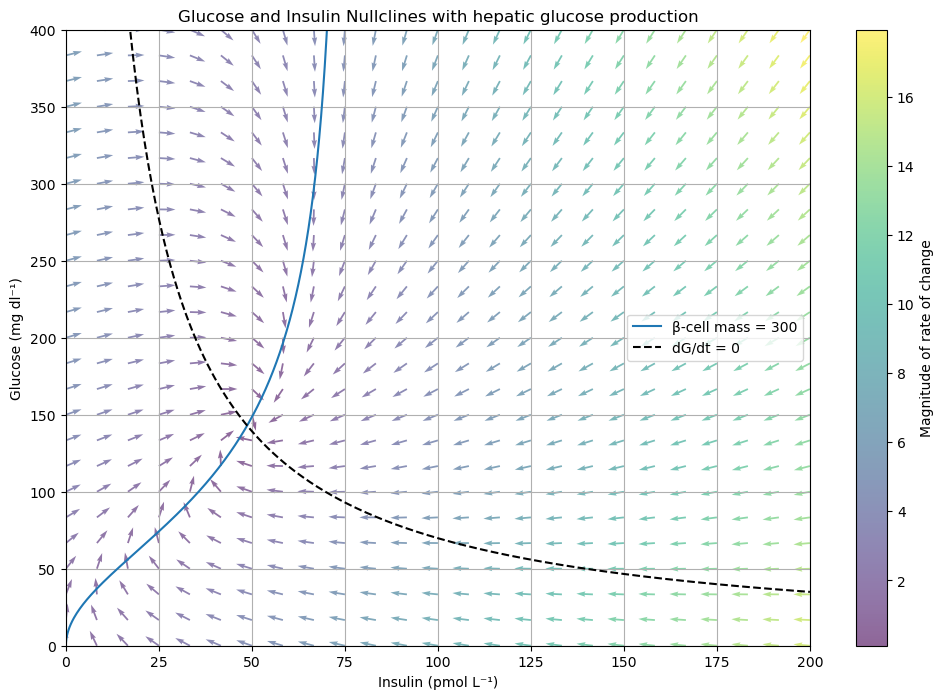
\includegraphics[width=0.9\textwidth]{Img/phase_300.png}
        \bicaption{模型\ref{model1}相图. }{Phase diagram of model \ref{model1}.}
    \end{minipage}
    \begin{minipage}[t]{0.5\textwidth}
        \centering
        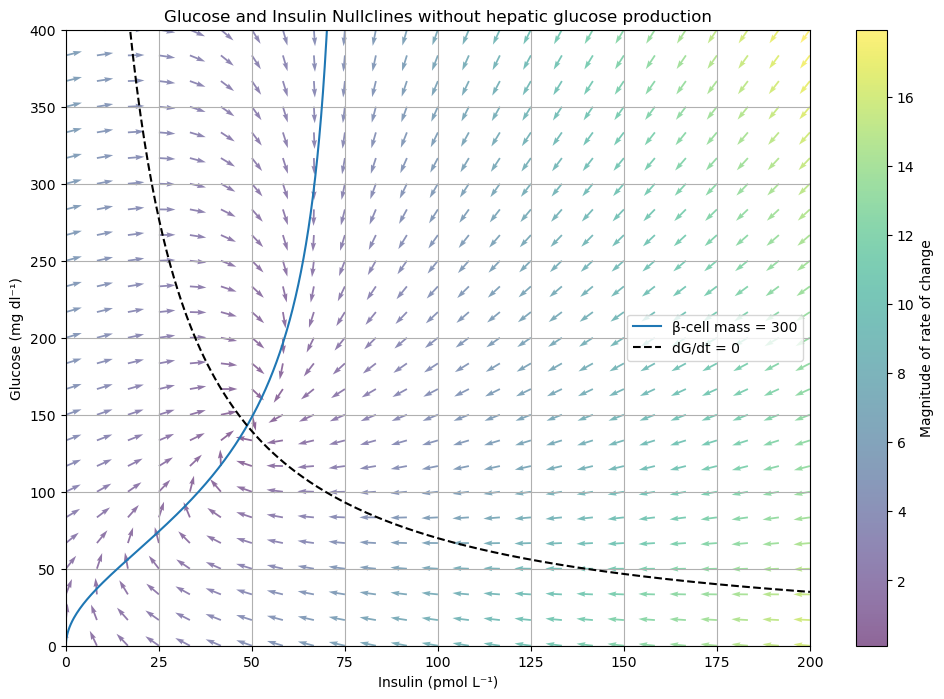
\includegraphics[width=0.9\textwidth]{Img/phase_hepatic.png}
        \bicaption{模型\ref{model2}相图. }{Phase diagram of model \ref{model2}.}
    \end{minipage}
\end{figure}
我们可以发现其差距很小,为了更好的训练模型,我们将侧重使用模型\ref{model2}来进行训练. 
由于连续血糖监测技术测量的是每15分钟的血糖数据,我们将每一段时间分为100段小部分来近似模型,因此我们可取$\Delta t = 0.15$. 

    
\section{连续血糖预测的算法和模型评估} 
我们采用如下算法对模型参数进行估计:
\begin{algorithm}[H]
    \caption{差分形式动力系统模型}
    \begin{algorithmic}[1]
    \State 初始化DFNet模型:
    \State \quad 将$a_0, a_1, a_2, b_1, b_2, b_3, I_0$设定为可学习参数
    \State \quad 将$\delta_t$设定为0.15
    \State 前向传播函数:
    \State \quad 输入:数据张量$x$
    \State \quad $length \gets x.size(0) - 1$
    \State \quad 初始化长度为$(length + 1) \times 100$的结果列表$res$
    \State \quad 将$res[0]$设为$x[0]$
    \State \quad 初始化长度为$(length + 1)$的$G$列表
    \State \quad 初始化长度为$(length + 1) \times 100$的$I$列表
    \State \quad 将$I[0]$设为$I_0$
    \For{$i$从0到$(length \times 100 + 99)$}
        \State $res[i + 1] \gets res[i] + 2 \times \delta_t \times (a0 - a1 \times res[i] - a2 \times res[i] \times I[i])$
        \State $I[i + 1] \gets I[i] + 2 \times \delta_t \times (b1 \times res[i]^2 / (res[i]^2 + b2^2) - b3 \times I[i])$
    \EndFor
    \For{$i$从0到$length$}
        \State $G[i] \gets res[i \times 100]$
    \EndFor
    \State 返回:堆叠后的$G$列表
    \State
    \Function{loss}{$x$}
        \State $pred \gets$ 前向传播函数($x$)
        \State \Return $x$与$pred$之间的均方误差
    \EndFunction
    \end{algorithmic}
    \end{algorithm}

    其中变量$length$表示需要得到的结果数据的长度, $res$表示通过动力系统模型预测得到的实时血糖值, $pred$表示在与输入的血糖数据对应的时间预测的血糖浓度, $LOSS$为损失函数. 

    我们用这个算法对模型进行训练,对于其中一组数据,模型\ref{model1}拟合结果如图\ref{fig:fit_1}:

    \begin{figure}[H]
        \centering
        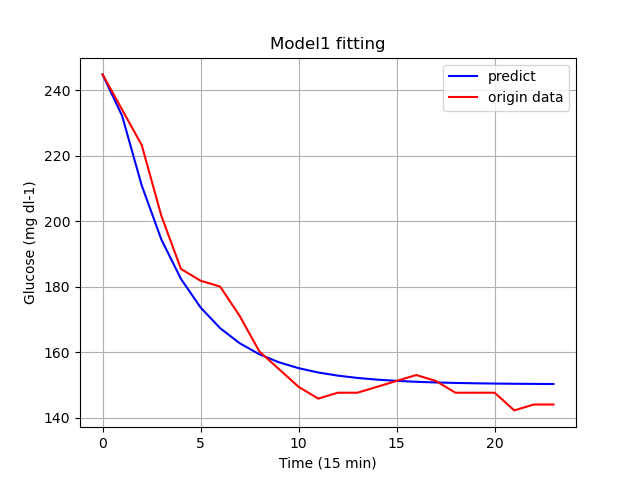
\includegraphics[width=0.7\textwidth]{Img/fit_1.png}
        \bicaption{模型\ref{model1}拟合结果. }{Fitting results of model \ref{model1}.}
        \label{fig:fit_1}
    \end{figure}
    我们可以看到模型\ref{model1}对数据的拟合效果较好,接下来我们将对该模型进行评估. 

    为了评估模型的预测效果,我们将使用均方误差(Mean Squared Error, MSE)评价指标. MSE是预测值与真实值之间差值的平方的均值,MSE越小,说明模型的预测效果越好. 我们将使用MSE来说明模型的预测效果. 对于同一个人的另一组数据,模型的预测效果如图\ref{fig:predict_1}:
    \begin{figure}[H]
        \centering
        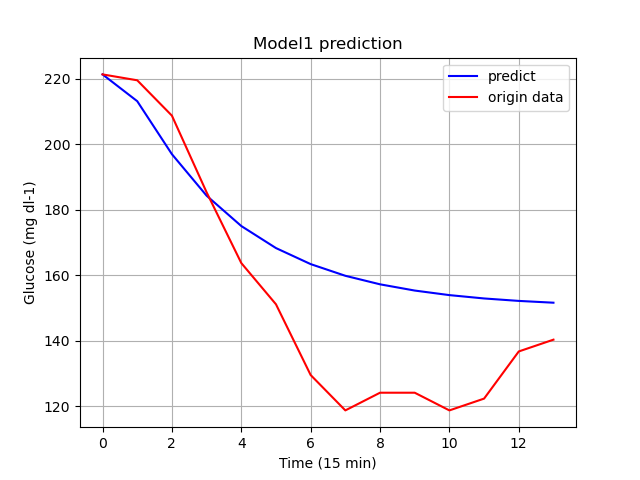
\includegraphics[width=0.7\textwidth]{Img/predict_1.png}
        \bicaption{模型\ref{model1}预测效果. }{Prediction results of model \ref{model1}.}
        \label{fig:predict_1}
    \end{figure}

    计算得到MSE为$574.86$. 

    对于模型\ref{model2},我们同样使用均方误差评价指标. 对于同样的数据,模型拟合结果如图\ref{fig:fit}:
    \begin{figure}[H]
        \centering
        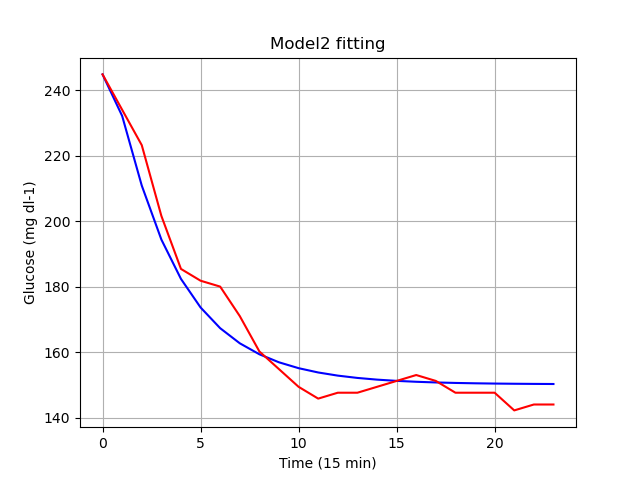
\includegraphics[width=0.7\textwidth]{Img/fit.png}
        \bicaption{模型\ref{model2}拟合结果. }{Fitting results of model \ref{model2}.}
        \label{fig:fit}
    \end{figure}

    我们使用与上一个模型评估所用的相同的数据,模型的预测效果如图\ref{fig:predict}:
    \begin{figure}[H]
        \centering
        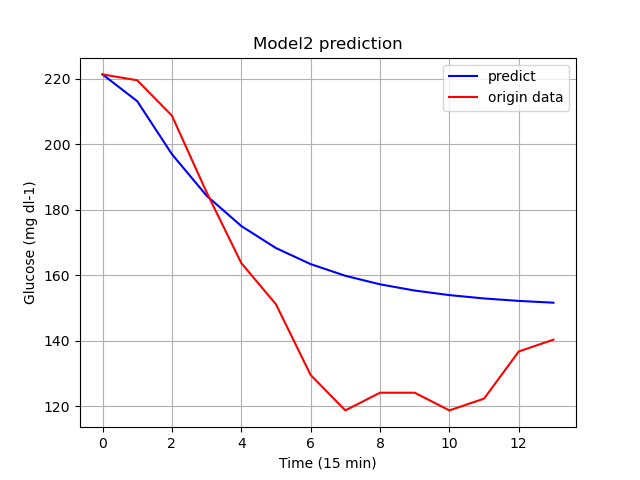
\includegraphics[width=0.7\textwidth]{Img/predict.png}
        \bicaption{模型\ref{model2}预测效果. }{Prediction results of model \ref{model2}}
        \label{fig:predict}
    \end{figure}

    计算得到MSE为$574.87$. 

    综上所述,模型\ref{model1}和模型\ref{model2}的预测效果相当,但模型\ref{model2}的参数更少,消耗计算量更少,因此我们更推荐选择模型\ref{model2}作为连续血糖预测模型. 由于人在不同时间段的不同举动都会对血糖浓度造成影响,我们不能通过动力系统模型完全描绘一个人一天中的各种举动,所以有些许误差是可以接受的. 

    \section{其他连续血糖预测模型}

    除了动力系统模型外,还有一些其他的连续血糖预测模型,例如基于大语言模型(Large Language Model, LLM)的预测模型\cite{healey2024leveraging}. LLM是一种基于神经网络的模型,可以通过学习大量的文本数据来预测下一个词的概率. 我们可以将血糖数据看作是一种时间序列数据,通过LLM模型来预测未来的血糖值. 但由于大语言模型需要大量的数据来训练,需要不少的前置测试数据,因此我们在这里不做详细讨论. 

    \section{动力系统模型的优势与不足}

    \subsection*{动力系统模型的不足之处}
    
    对比大语言模型,由于动力系统模型并不能完全考虑到人体内部的各种生理过程,比如人体吸收和消耗葡萄糖的速率并不能视为一个常数,但目前又没有一个较好的模型来衡量,所以说数据预测并不那么准确,而大语言模型可以通过大量的数据来学习人体的各种生理过程,对于一个人的生活习惯,饮食习惯等都可以通过大语言模型来学习,因此大语言模型在预测效果上会更好一些. 

    \subsection*{动力系统模型的优势}

    但由于当人们在得知自己已患有糖尿病或有得糖尿病的风险时,可能会改变自身的习惯,随着锻炼,饮食习惯的改变,大语言模型的预测效果会逐渐变差,由于大语言模型的训练需要大量的数据,并且是针对个人个性化的,因此在这种情况下,动力系统模型的预测效果会更好一些. 在这里动力系统模型就体现出了其优势:短期有效,方便更新. 
